\myChapter{Distributed Evolutionary Algorithms}\label{chap:MOS}
\minitoc\mtcskip
\vfill
\lettrine{E}{volutionary} 
\section{Parallel and Distributed Evolutionary Algorithms models}
\lettrine{T}{here} are different ways to parallelize the EAs, being the most extended:

\subsection{Farming model (centralized EAs)} 
A central node coordinate several slave nodes. The central node executes the EA in a sequential way, but distributes the individuals of the population to the slaves just for being evaluated. An example can be seen in \cite{NUCLEAR}, where slave nodes evaluates fitness function for simullation of nuclear devices.
\subsection{Island model (distributed EAs)}
A number of nodes executes simultaneously the EA, working with different sub-populations at the same time. Each certain number of generations is interchanged (migrated) between populations. Figure \ref{fig:islands} shows this model with a ring topology.

\begin{SCfigure}[20][htb]
\centering
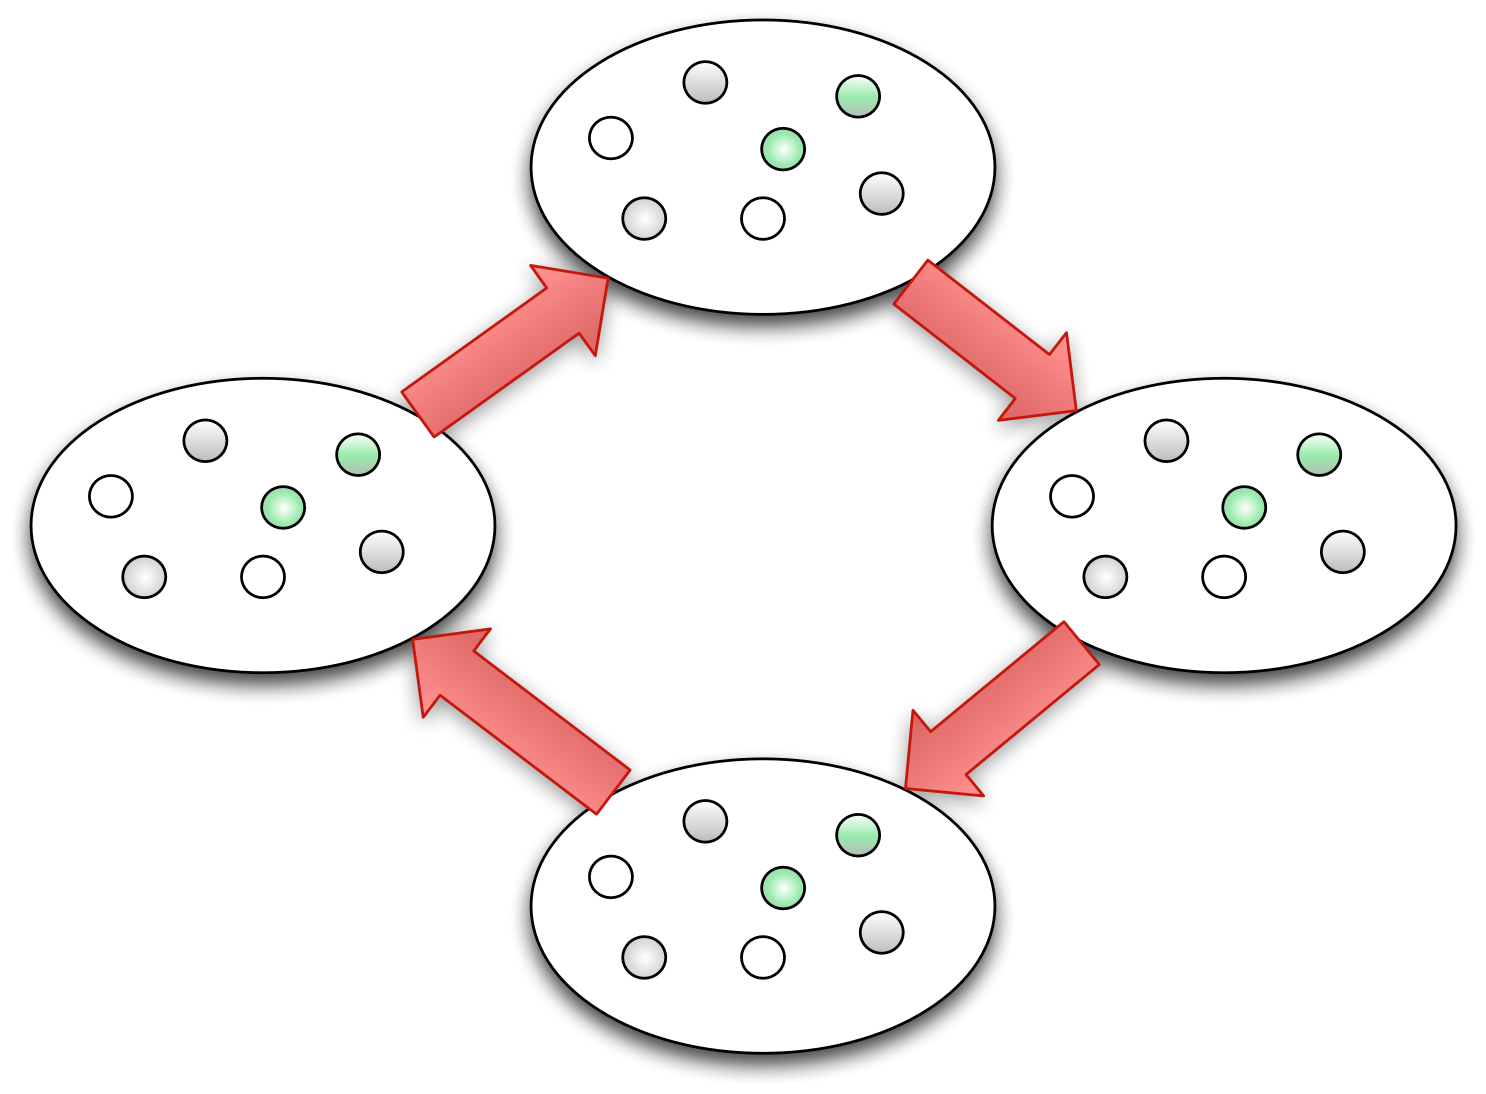
\includegraphics[width=26pc]{gfx/ring.jpg}
\caption{Island model scheme using a neighborhood ring topology.}
\label{fig:islands}
\end{SCfigure}

\subsection{Cellular EAs (fine grain EAs)}
Each node has one individual of the population, and selection and reproduction is limited with the individuals of the neighbourhood of the node \cite{CELLULAR}. Usually a bi-dimensional grid is used for topology. 

\subsection{Non conventional methods}




\section{Frameworks for Evolutionary Algorithms}

In \cite{GENERICITY05}, \person{Gagn{\'e}and Parizeau} presented six criteria for qualify EA frameworks: generic representation, fitness, operator, model, parameters management and configurable output. In this work we show how SOA follows these lines of genericity, but can also extend them:
\begin{itemize}
\item Genericity in the service interfaces: service interfaces are established to create new implementations. Furthermore, these interfaces must be abstract enough to avoid their modification.
\item Programming language independence: for example, services implemented in Java can use services implemented in C++ and vice-versa.
\item Distribution transparency: it is not mandatory to use a specific library for the distribution, or modify the code to adapt the existing operators.
\item Flexibility: easy to add and remove elements to use the self-adaptation or other mechanisms.
\end{itemize}

Even as SOA is used extensively in software development, it is not widely accepted in the main EA software. 

\subsection{Object Oriented Frameworks}
Firstly, there exist
Object Oriented frameworks, such as Al\-go\-rithm::Evo\-lu\-tionary \citep{PERL},
\definicion{JCLEC}{Java Class Library for Evolutionary Computation} \citep{JCLEC} or jMetal \citep{JMETAL}. 
 Users implement specific interfaces of these frameworks (such as {\em
   individual} or {\em crossover}) and they group them in the source
 code. For example, creating an operator object that groups several
 operators. However, these frameworks are not compatible among them.
 For example, the operators created in JCLEC can not be used in jMetal
 (despite both are programmed in Java). Also, they can not control the
 services (operators) outside the source code.

\subsection{Parallel frameworks} 
Parallelism and distribution are added in other frameworks, such as
MALLBA \citep{MALLBA}, \definicion{DREAM}{Distributed Resource Evolutionary Algorithm Machine} \citep{DREAM} or \definicion{ECJ}{Evolutionary Computation in Java} \citep{ECJ}, but
using external libraries (such as \definicion{MPI}{Message Passing Interface} or \definicion{DRM}{Distributed Resource Machine}), so the code that uses these
libraries is mixed with the algoritmh's code.


 Even being distributed, these frameworks can not communicate with each other. HeuristicLab \citep{HEURISTICLAB} is one of the few plug-in and service oriented frameworks. It uses web services for communication, but just to distribute the load, after consulting a central database of available jobs. Finally, the only service oriented optimization framework is GridUFO \citep{GRIDUFO}, but it only allows the modification of the objective function and the addition of whole algorithms, without combining existing services.  Table \ref{tablaframeworks} shows a summary of the previous frameworks.


\begin{SCtable}[][t]
\resizebox{11cm}{!}{
\begin{tabular}{llllll}
\hline
\rowcolor{colorCorporativoSuave}Name		&  Design 	 & Language 	& Distribution 	& License  		& Other	\\
\hline\hline
\rowcolor{colorCorporativoMasSuave}ECJ		& OO		& Java		& Sockets   	& Academic Free Lic. 	& Recently updated		\\
\rowcolor{colorCorporativoSuave}MALLBA		& OO		& C++		& MPI		& Freeware		& No new versions	\\
\rowcolor{colorCorporativoMasSuave}jMetal		& OO		& Java		& N/A		& GNU/LGPL 		&		\\
\rowcolor{colorCorporativoSuave}DREAM		& OO		& Java		& DRM		& GNU/GPL   		& No new versions		\\
\rowcolor{colorCorporativoMasSuave}ParadiseEO	& OO		& C++		& MPI		& CeCILL	   	&		\\
\rowcolor{colorCorporativoSuave}HeuristicLab	& OO/PO 	& .NET		& Web-Services	& GNU/GPL		& Recently updated			\\
\rowcolor{colorCorporativoMasSuave}METCO		& OO		& C++		& MPI		& N/A	   		&	\\
\rowcolor{colorCorporativoSuave}JCLEC		& OO		& Java		& N/A		& GNU/GL   		&	\\
\rowcolor{colorCorporativoMasSuave}Algorithm::Evol.& OO		& Perl		& N/A		& GNU/GPL  		& 	\\
\rowcolor{colorCorporativoSuave}GridUFO		&SO		& Java		& Web Services	& N/A  			& 	\\
\hline
%OSGiLiath	&OO/SO/PO 	& 2010			& Java		& Distributed OSGi	& GNU/GPL  	& Lifecycle management	\\
\end{tabular}
}
\caption{Comparison of EA frameworks. OO=Object-Oriented, SO=Service Oriented, PO=Plug-in Oriented}
\label{tab:frameworks}
\end{SCtable}

In brief, although these frameworks follows the six criteria for genericity proposed in \cite{GENERICITY05}, they present some shortcomings when it is needed to develop
or add new features: the user is forced to modify the source code
or stop the execution to add new functionalities (like load balancing,
dynamic control of operators, or an user interface). The authors should
improve their frameworks adding SOA technologies in order to facilitate the
communication and integration among them. As \person{Parejo \etal}  suggest in \cite{SURVEYMOFS}, a standardization of the presented (and other) frameworks should be carried out.

\begin{SCtable}[][!hb]
\begin{tabular}{|A|}
\hline
AQUI PUEDE IR EL ALGORITMO
\\
\hline
\end{tabular}\caption[Criterios generales calidad]{Criterios generales para la evaluaci�n de la calidad de los algoritmos de extracci�n de bordes.}\label{tab:criteriosGenerales}
\end{SCtable}
